\documentclass[11pt,a4paper]{article}
\usepackage[spanish,es-nodecimaldot]{babel}	% Utilizar español
\usepackage[utf8]{inputenc}					% Caracteres UTF-8
\usepackage{graphicx}						% Imagenes
\usepackage[hidelinks]{hyperref}			% Poner enlaces sin marcarlos en rojo
\usepackage{fancyhdr}						% Modificar encabezados y pies de pagina
\usepackage{float}							% Insertar figuras
\usepackage[textwidth=390pt]{geometry}		% Anchura de la pagina
\usepackage[nottoc]{tocbibind}				% Referencias (no incluir num pagina indice en Indice)
\usepackage{enumitem}						% Permitir enumerate con distintos simbolos
\usepackage[T1]{fontenc}					% Usar textsc en sections
\usepackage{amsmath}						% Símbolos matemáticos
\usepackage{verbatim}

% Comando para poner el nombre de la asignatura
\newcommand{\asignatura}{Programación Técnica y Científica}
\newcommand{\autor}{Vladislav Nikolov Vasilev}
\newcommand{\titulo}{Práctica 2}
\newcommand{\subtitulo}{Robótica}

% Configuracion de encabezados y pies de pagina
\pagestyle{fancy}
\lhead{\autor{}}
\rhead{\asignatura{}}
\lfoot{Grado en Ingeniería Informática}
\cfoot{}
\rfoot{\thepage}
\renewcommand{\headrulewidth}{0.4pt}		% Linea cabeza de pagina
\renewcommand{\footrulewidth}{0.4pt}		% Linea pie de pagina

\begin{document}
\pagenumbering{gobble}

% Pagina de titulo
\begin{titlepage}

\begin{minipage}{\textwidth}

\centering

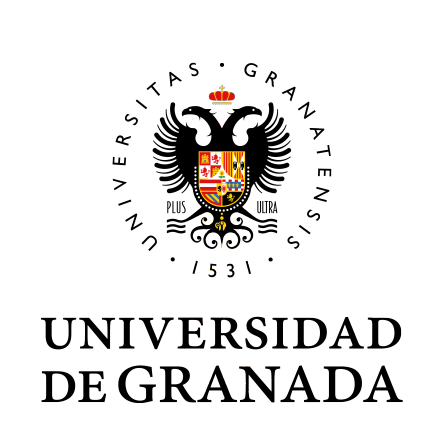
\includegraphics[scale=0.5]{img/ugr.png}\\

\textsc{\Large \asignatura{}\\[0.2cm]}
\textsc{GRADO EN INGENIERÍA INFORMÁTICA}\\[1cm]

\noindent\rule[-1ex]{\textwidth}{1pt}\\[1.5ex]
\textsc{{\Huge \titulo\\[0.5ex]}}
\textsc{{\Large \subtitulo\\}}
\noindent\rule[-1ex]{\textwidth}{2pt}\\[3.5ex]

\end{minipage}

\vspace{0.5cm}

\begin{minipage}{\textwidth}

\centering

\textbf{Autor}\\ {\autor{}}\\[2.5ex]
\textbf{Rama}\\ {Computación y Sistemas Inteligentes}\\[2.5ex]
\vspace{0.3cm}


\includegraphics[scale=0.3]{img/etsiit.jpeg}

\vspace{0.7cm}
\textsc{Escuela Técnica Superior de Ingenierías Informática y de Telecomunicación}\\
\vspace{1cm}
\textsc{Curso 2019-2020}
\end{minipage}
\end{titlepage}

\pagenumbering{arabic}
\tableofcontents
\thispagestyle{empty}				% No usar estilo en la pagina de indice

\newpage

\setlength{\parskip}{1em}

\section{Objetivo de la práctica}

El principal objetivo de esta práctica es hacer que un robot sea capaz de diferenciar
las piernas de las personas de objetos que no son piernas, como podrían ser por
ejemplo cilindros. Para ello, se ha propuesto utilizar un simulador donde se dispondrá
de un robot con un sensor láser y una cámara. Se tomarán primeramente datos y después
de procesarlos se entrenará un modelo de \textit{machine learning} que clasifique la
información como ``pierna'' y ``no pierna''. El modelo que se propone utilizar es un
\texttt{SVM}, y hay que escoger la mejor variante de dicho modelo comparando una serie
de \textit{kernels} e hiperparámetros. Una vez que se tenga el modelo definitivo, se utilizará
una escena de test para ver qué tan bien lo hace con datos nuevos. Finalmente se creará
un archivo en formato \texttt{HTML} que contendrá una tabla donde se mostrarán fotos de los
objetos detectados, además de la distancia a la que están del robot y de la clase real y
de la predicha.

En esta memoria se expondrá que \textit{scripts} se han utilizado, qué funcionalidad tiene cada
uno y se describirá brevemente lo que se ha ido haciendo.

\section{Captura de los datos}

Lo primero que se ha hecho ha sido capturar los datos. Para hacerlo, se ha creado un
\textit{script} llamado \textbf{capturar.py}, cuyo funcionamiento puede resumirse en
que pide al usuario el nombre del archivo de salida, el directorio donde quiere que
se guarde el fichero, el número de ciclos que se quiera leer y cuánto tiempo se tiene
que esperar entre lectura y lectura. Una vez hecho esto, se establece conexión
con el servidor de V-REP activo y se crea el directorio de salida y se cambia
el entorno de trabajo a este directorio. Una vez hecho esto, se toman los datos durante
tantos ciclos como se ha especificado anteriormente, haciendo una pausa entre cada captura
en la cantidad de segundos especificada. En cada lectura se van guardando los datos en el
fichero de salida. Además, se toma una captura de la cámara en la primera y en la última toma
de datos. Finalmente, se finaliza la conexión.

Para modularizar el código, el \textit{script} se ha estructurado en funciones. Estas
funciones se describen a continuación:

\begin{itemize}[label=\textbullet]
	\item \texttt{establecer\_conexion}: Establece la conexión con el servidor
	de V-REP activo y devuelve un ID del cliente. En caso de que no se pueda conectar,
	se finaliza la ejecución del \textit{script}.
	\item \texttt{obtener\_camara\_handler}: Obtiene un \textit{handler} de la cámara
	e inicializa la cámara y el sensor láser. Devuelve la referencia al \textit{handler}
	de la cámara para usos futuros.
	\item \texttt{init\_entorno}: Combina las dos funciones anteriores en una y devuelve
	tanto el ID del cliente como el \textit{handler} de la cámara.
	\item \texttt{procesar\_ciclo}: Esta función hace una captura del sensor laser y obtiene
	información sobre los puntos detectados en los ejes $X$ e $Y$. Una vez hecho esto, crea
	un diccionario que contiene información sobre la iteración actual y los puntos detectados
	en los dos ejes anteriores, con el mismo formato que el que se puede ver en los ficheros
	de ejemplo.
	\item \texttt{capturar\_guardar\_imagen}: Esta función hace una captura de lo que ve la
	cámara de la misma forma que se hacía en el código de ejemplo. Guarda el resultado
	en un fichero con un nombre específico.
	\item \texttt{stop\_simulacion\_conexion}: Con esta función se detiene la simulación
	que se está haciendo y se cierra la conexión con el servidor.
\end{itemize}

Para capturar los datos, se han creado 4 escenas: una con una persona de pie, una con una persona
sentada, una con un par de cilindros más pequeños que las piernas de una persona y otra
con un par de cilindros más grandes que las piernas de una persona. Para cada caso se han tomado
capturas de cerca, a distancia media y de lejos. Este proceso se puede ver a continuación:

\begin{figure}[H]
\centering
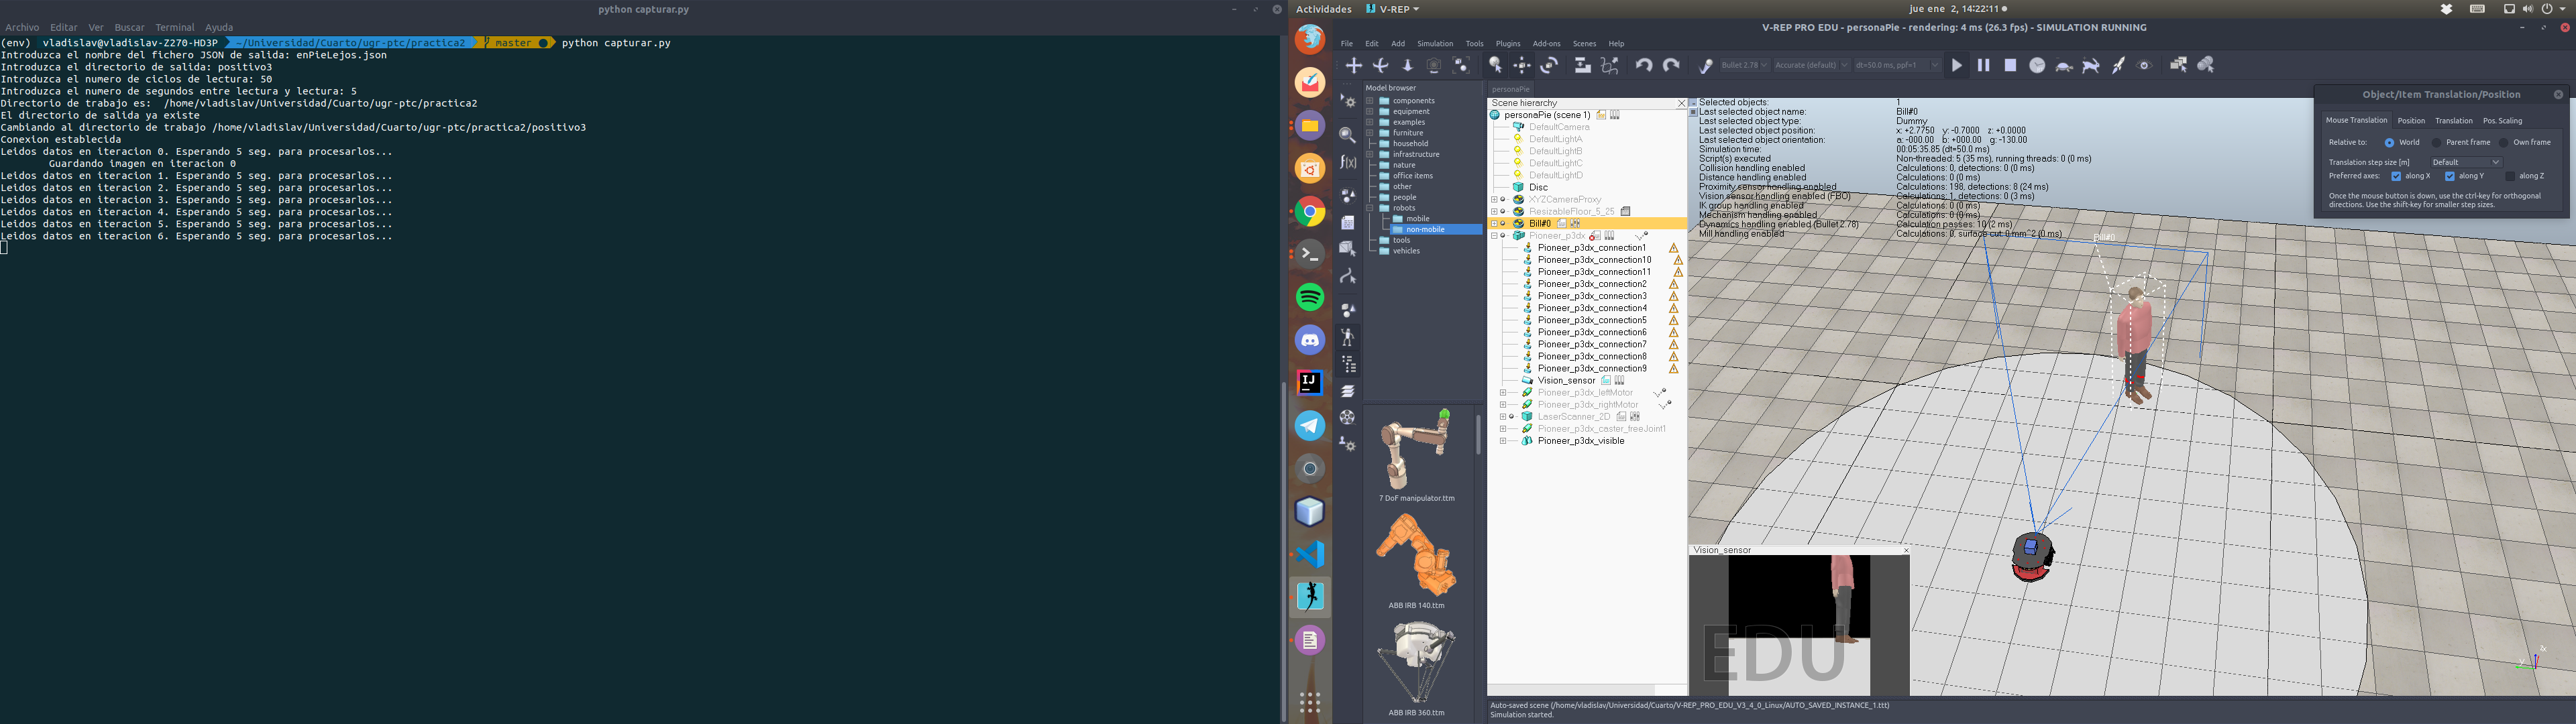
\includegraphics[scale=0.1]{img/pie2.png}
\caption{Captura de datos con persona de pie.}
\end{figure}

\begin{figure}[H]
\centering
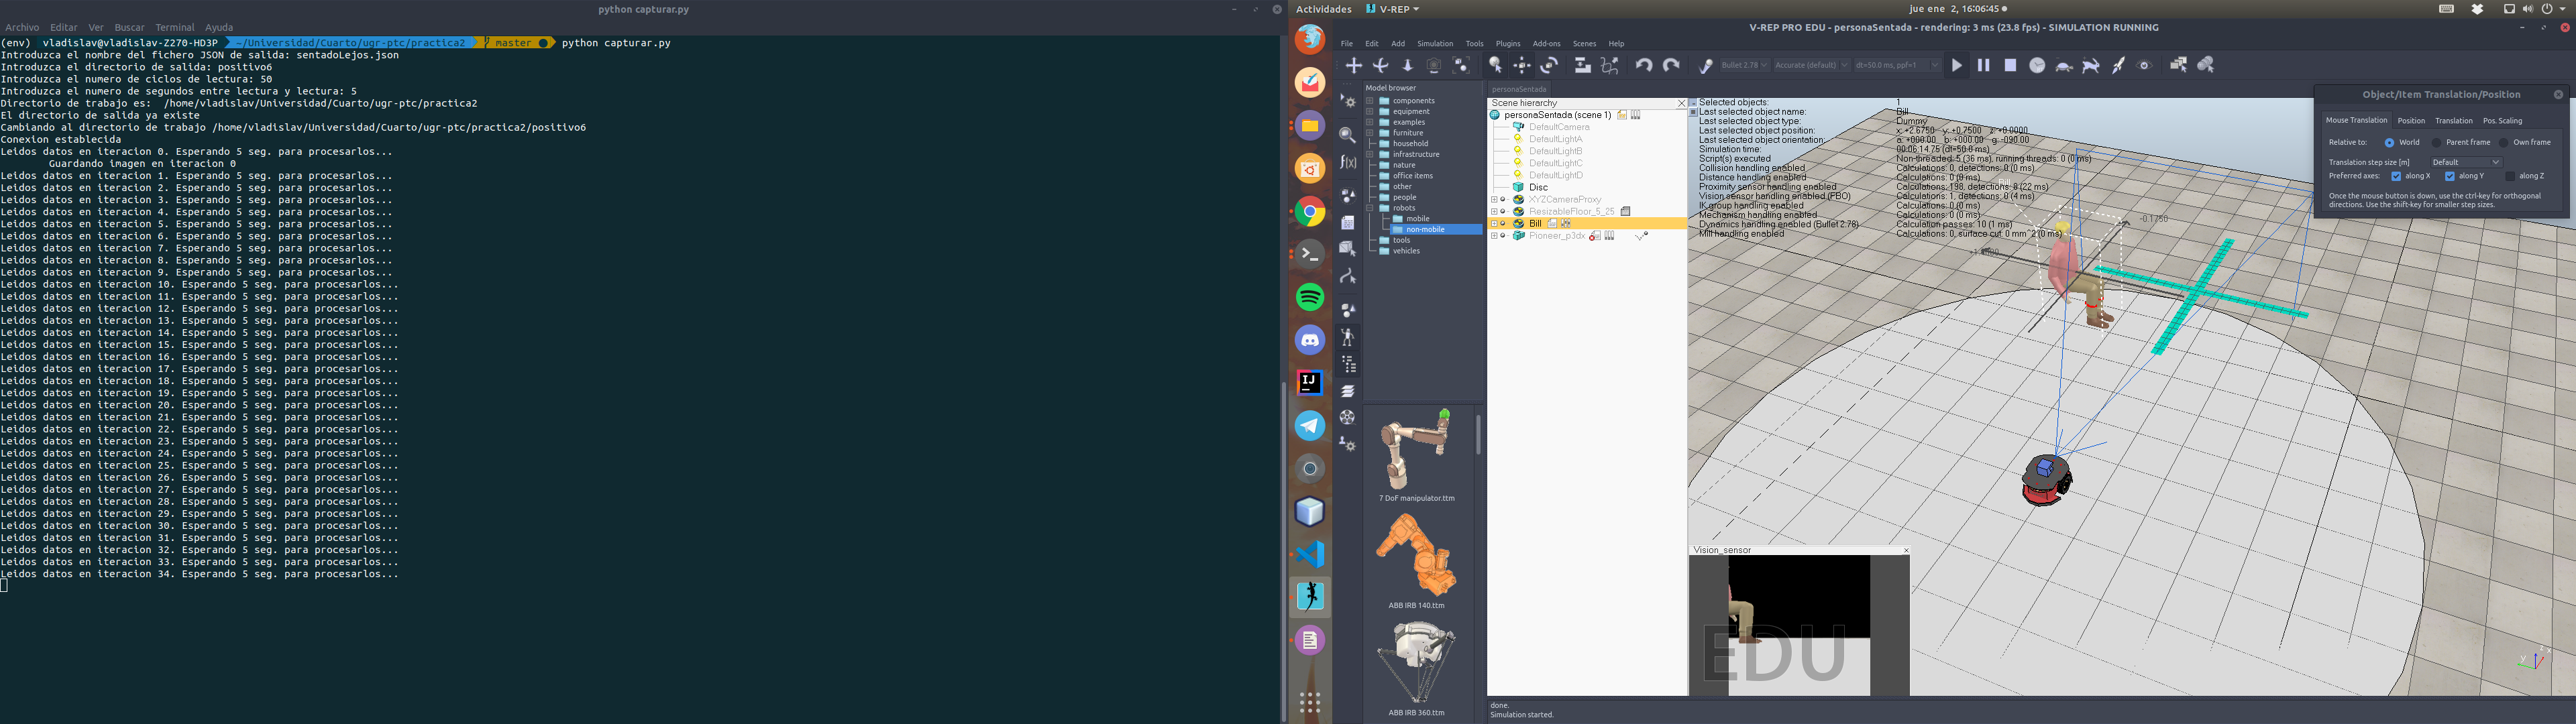
\includegraphics[scale=0.1]{img/sentado2.png}
\caption{Captura de datos con persona sentada.}
\end{figure}

\begin{figure}[H]
\centering
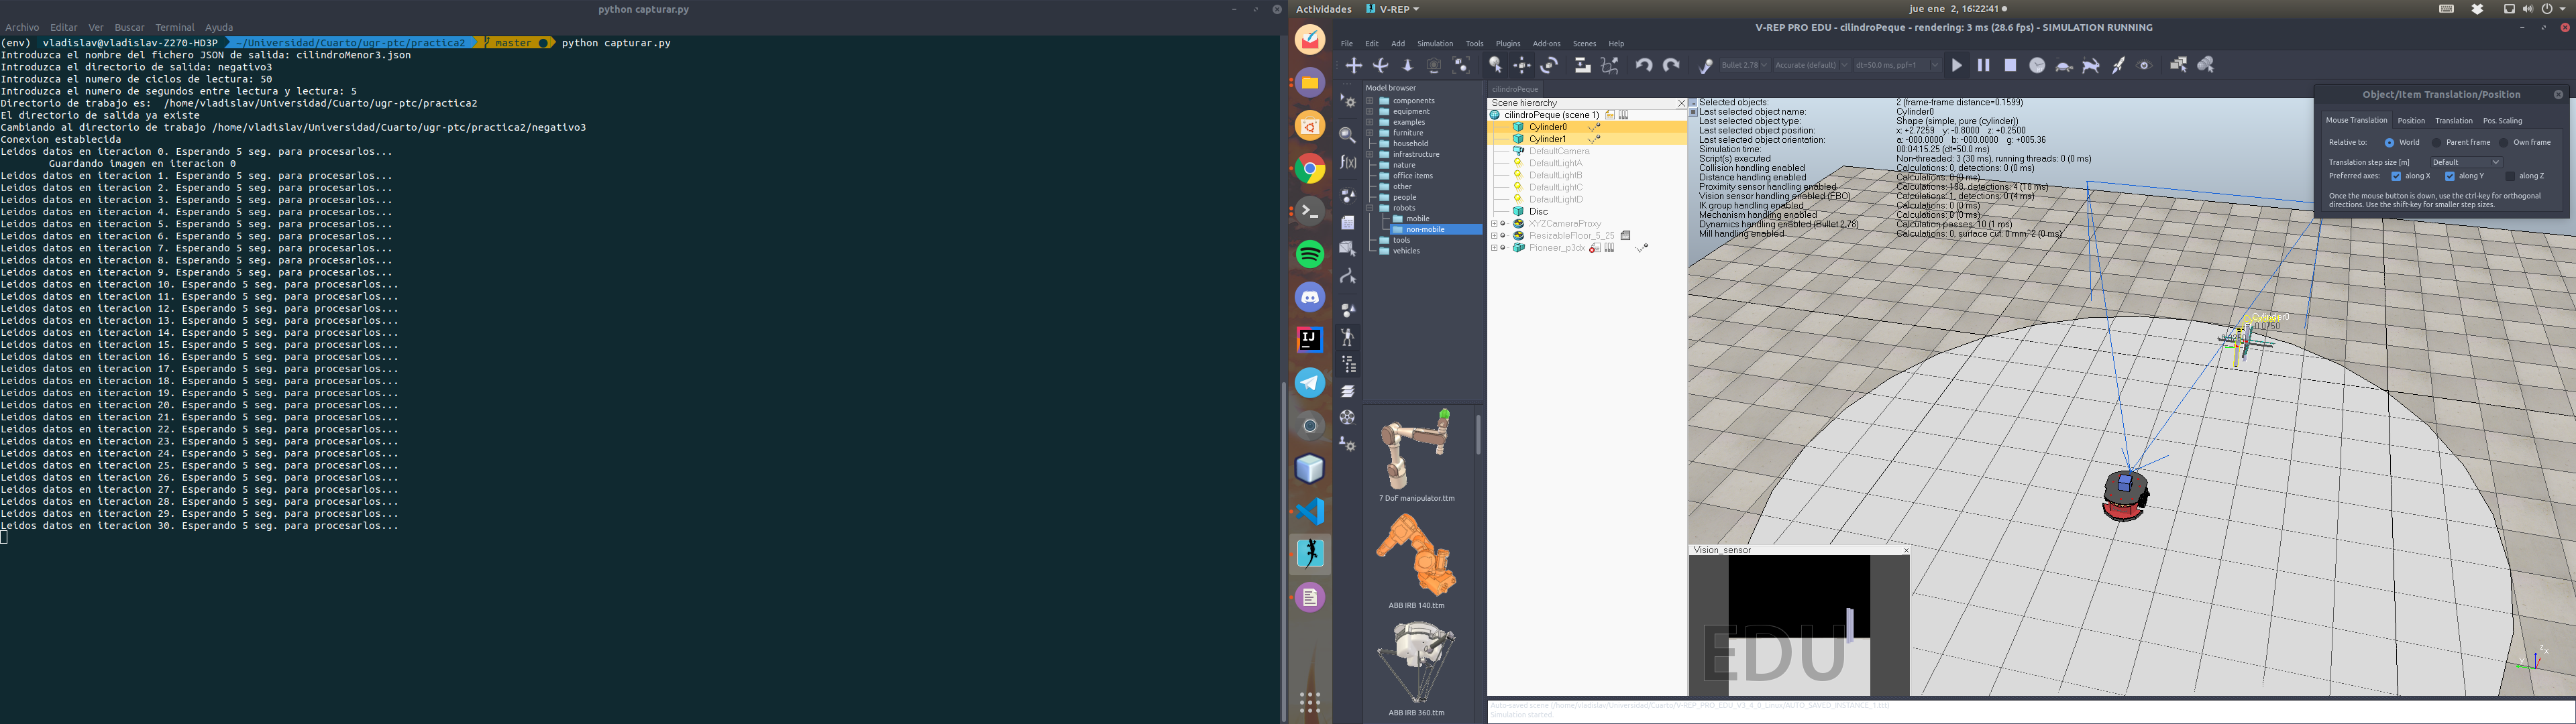
\includegraphics[scale=0.1]{img/peque2.png}
\caption{Captura de datos con par de cilindros pequeños.}
\end{figure}

\begin{figure}[H]
\centering
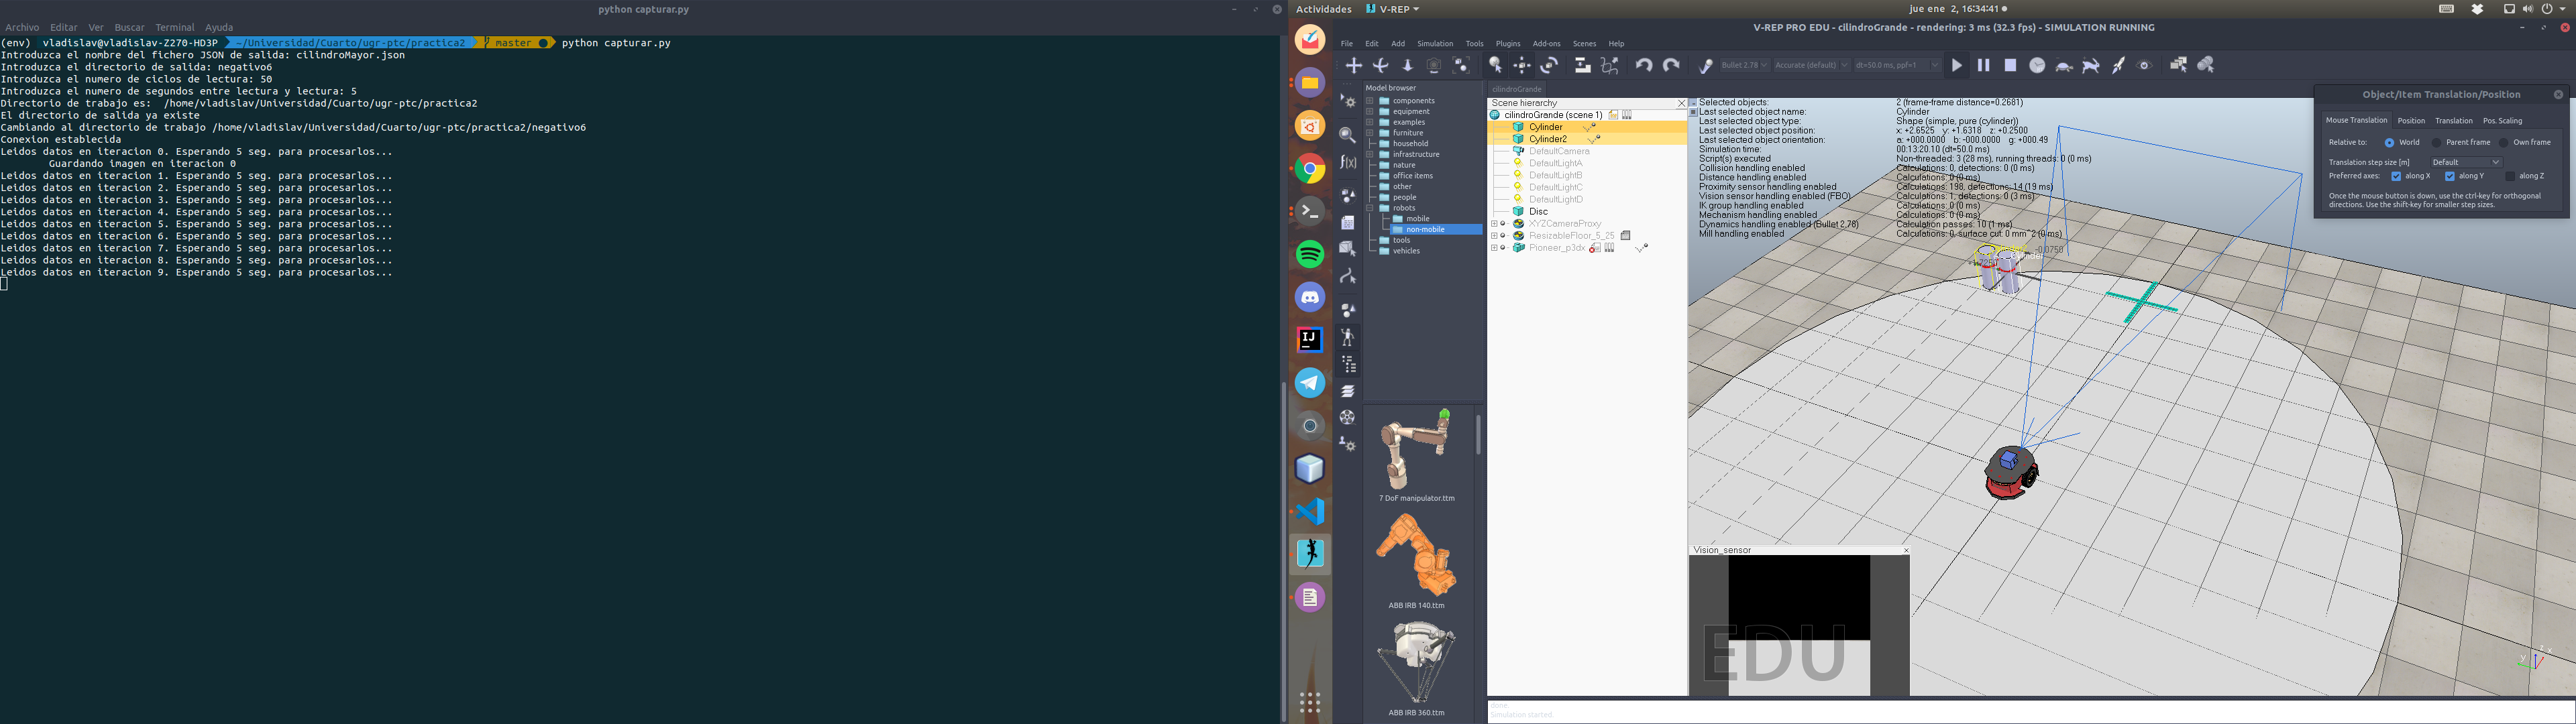
\includegraphics[scale=0.1]{img/grande2.png}
\caption{Captura de datos con par de cilindros grandes.}
\end{figure}

Como se puede ver, también se ha puesto un círculo en el suelo de radio $3.5$, el cuál sirve
de guía a la hora de tomar las capturas de los datos, para no salirse del radio especificado.

\section{Agrupación de los puntos en clusters}

Una vez que se han tomado los datos, hace falta agrupar los puntos en clusters. Para
ello se ha creado un \textit{script} llamado \textbf{agrupar.py} el cuál se encarga
precisamente de eso.

El funcionamiento general se resumen en que toma todos los directorios de ejemplos positivos
y de ejemplos negativos y crea clusters a partir de la información de cada tipo de directorio,
según el formato que se ha especificado.
Finalmente, guarda los ejemplos negativos en un fichero en formato \texttt{JSON} y los positivos
en otro, teniendo por tanto la información separada.

Para crear los clusters es necesario establecer el número mínimo de puntos que lo pueden formar,
el máximo y la distancia que puede haber, como máximo, entre dos puntos consecutivos.
En un primer instante había establecido que el \textbf{número mínimo de puntos} fuese 3,
el \textbf{número máximo de puntos} fuese 25 y la \textbf{distancia máxima entre dos puntos consecutivos}
fuese $0.03$. Sin embargo, estos valores se modificarán más adelante, aunque se comentará
en la sección correspondiente.

De nuevo, tal y como se hizo ante, se ha estructurado el fichero en funciones, las cuáles
se pueden ver a continuación:

\begin{itemize}[label=\textbullet]
	\item \texttt{obtener\_cluster\_datos}: Esta función se encarga de extraer un único
	cluster a partir de un conjunto de puntos. Recorre el \textit{array} de puntos
	proporcionado, el cuál está compuesto por coordenadas $(x, y)$, y va añadiendo
	los puntos consecutivos a una lista, siempre y cuando la distancia de un punto
	al siguiente no supere el umbral, haya menos puntos que el máximo permitido en la
	lista y no se supere la longitud del \textit{array} de entrada (ya que se está
	recorriendo con índices).
	\item \texttt{procesar\_clusters\_muestra}: Esta función procesa una muestra de datos,
	generando los clusters que se pueden encontrar en el conjunto de puntos. Utiliza la
	función anterior para determinar los clusters uno por uno y al final los
	junta en una única lista. Se acepta un cluster siempre y cuando el número de puntos
	supere al mínimo requerido. La función está pensada para que pueda recibir la inforamción
	como un diccionario de \texttt{Python}, de forma que se pueda reutilizar más adelante.
	Por tanto, si se le quiere pasar información que está en formato \texttt{JSON}, se tiene
	que cargar antes.
	\item \texttt{procesar\_clusters\_fichero}: Con esta función se pueden procesar
	los clusters de un fichero determinado. Hace uso de la función anterior, y junta
	los clusters de cada muestra en una única lista.
	\item \texttt{procesar\_clusters\_directorios}: Con esta función se pueden obtener
	los clusters de todos los archivos de un conjunto de directorios del mismo tipo.
	Para ello, se utiliza la función anterior, la cuál procesa cada fichero de forma
	individual. Se devuelve una lista con los clusters encontrados para todos los
	directorios del mismo tipo.
	\item \texttt{generar\_informacion\_cluster}: Esta función permite generar la información
	de salida de los clusters, en el formato especificado. Recibe la lista de clusters y construye
	una lista con diccionarios con el mismo formato.
	\item \texttt{guardar\_clusters}: Esta función permite guardar los clusters en un
	archivo con un nombre determinado. Para generar la información, utiliza la función
	anterior. Después, la transforma a formato \texttt{JSON} y la escribe en el fichero
	de salida.
\end{itemize}

\section{Extracción de características}

Una vez que se han agrupado los puntos en clusters, se pueden extraer características,
las cuáles serán útiles a la hora de entrenar el clasificador. Dichas características son
el \textbf{perímetro}, la \textbf{anchura} y la \textbf{profundidad} del cluster.
Para conseguir dicha tarea
se ha creado un \textit{script} llamado \textbf{caracteristicas.py}. Este programa lee
los ficheros creados anteriormente y genera las características para cada uno, guardando
la información de forma separada tal y como se hacía antes. Los datos tienen el formato
de salida especificado en el enunciado. Una vez hecho esto, carga los dos ficheros
que acaba de generar y crea un archivo en formato \texttt{CSV} donde se juntan los
datos de las dos clases, escribiendo primero los ejemplos de ``no pierna'' y luego
los de ``pierna''.

El fichero se ha estructurado en las siguientes funciones:

\begin{itemize}[label=\textbullet]
	\item \texttt{calcular\_perimetro}: Función con la que se calcula el perímetro
	para un cluster determinado.
	\item \texttt{calcular\_anchura}: Función con la que se calcula la anchura para
	un cluster determinado.
	\item \texttt{calcular\_profundidad}: Función que calcula la profundidad de un
	cluster determinado. Para hacerlo, se utiliza el producto vectorial, ya que
	simplifica bastante los cálculos. Se hace dicha operación para cada punto
	del cluster excepto para el primero y el último y se escoge el resultado más
	grande (es decir, la mayor distancia).
	\item \texttt{calcular\_caracteristicas}: Función con la que se calculan las
	tres características anteriormente mencionadas. Utiliza las tres funciones anteriores.
	\item \texttt{generar\_caracteristicas\_clusters\_muestra}: Esta función se
	utiliza para generar las caracteristicas de un conjunto de clusters de una muestra
	determinada. No se usa directamente en el programa, pero se deja la función para usos
	futuros, los cuáles se comentarán más adelante. Utiliza la función anterior para
	calcular las características.
	\item \texttt{generar\_caracteristicas\_clusters}: Esta función se utiliza para
	generar las características de un conjunto de clusters a partir de la información
	leída de un fichero. Utiliza la función para calcular características anteriormente
	mencionada. Guarda los resultados en un archivo con formato \texttt{JSON}.
	\item \texttt{escribir\_clase}: Esta función permite escribir los datos de uno de
	los ficheros generados con la función anterior a un fichero con formato \texttt{CSV}.
	\item \texttt{generar\_dataset}: La función permite generar el conjunto de datos
	que se utilizará para entrenar el clasificador. Utiliza la función anterior para
	escribir en el mismo fichero los ejemplos negativos primero y después los positivos.
\end{itemize}

\section{Entrenamiento de un clasificador \texttt{SVM}}

Una vez que se han generado las características y se han guardado en un fichero, podemos
entrenar un modelo de \textit{machine learning} para poder detectar piernas. Tal
y como se dijo anteriormente, se va a entrenar un \texttt{SVM}, y se van a probar
una serie de \textit{kernels} distintos para ver cuál se adapta mejor. Cuando se conozca
la mejor opción, se ajustarán los hiperparámetros para ver cuáles son los mejores valores.
Los \textit{kernels} que vamos a probar son uno lineal, uno polinómico de grado 2, uno de
grado 3, uno de grado 4 y un \textit{kernel} de base radial, también conocido como \texttt{rbf}.

El proceso general para determinar el mejor modelo y entrenarlo va a ser el siguiente:

\begin{enumerate}
	\item \textbf{Dividir el dataset anteriormente generado en dos conjuntos: uno de de entrenamiento
	y uno de validación}. Entrenaremos nuestro modelo con los datos de entrenamiento y estudiaremos
	su comportamiento con los datos de validación.
	\item\textbf{Hacer un primer estudio del comportamiento de los distintos modelos utilizando validación
	cruzada}. De esta forma, se dividirá el conjunto de entrenamiento en
	$n$ particiones (muy importante que se conserve la proporcionalidad de las clases). Se entrenará
	el modelo con $n-1$ particiones y la restante se utilizará para validar. Este proceso se
	repite $n$ veces, utilizando todas las particiones para validar. De esta forma, obtendremos
	$n$ resultados de \textit{accuracy}, y al promediar tendremos una primera aproximación
	de los resultados que se podrían obtener con el conjunto de validación real, o lo que es
	lo mismo, al intentar predecir datos que nunca antes había visto. En este caso, se utilizarán
	5 particiones, ya que se estima que es una cantidad razonable para la cantidad de datos de la
	que se dispone.
	\item \textbf{Ajustar los modelos con el conjunto de entrenamiento y validar los resultados con el
	conjunto de validación}. De esta forma veremos qué resultados se obtienen con el conjunto
	de validación que tenemos, para ver cómo de bien funcionan y si los resultados se aproximan
	a lo que habíamos obtenido con la validación cruzada. Además, de esta forma podremos obtener
	otras métricas aparte de la \textit{accuracy}, como por ejemplo la matriz de confusión, la cuál
	nos permitirá ver cómo se comporta el modelo a la hora de predecir los datos de cada clase (cuántos
	predice bien y cuántos no), la precisión (la capacidad de no clasificar ejemplos positivos como
	negativos) y el \textit{recall} (la capacidad para encontrar los ejemplos verdaderos de cada clase).
	\item \textbf{Escoger el mejor modelo y ajustar los hiperparámetros}. Para escoger dicho modelo, vamos
	a fijarnos en los resultados que se han obtenido en los dos pasos anteriores. Aquel modelo
	que tenga una mejor \textit{accuracy} y unos mejores resultados en el resto de métricas podrá
	ser considerado como el mejor. En cuanto al ajuste de hiperparámetros, en este caso vamos
	a ajustar el parámetro $C$ del modelo, el cuál mide cuánto se penalizan los puntos que caen
	dentro del margen del modelo (recordemos que \texttt{SVM} intenta encontrar el mejor separador,
	dejando la mayor cantidad de margen posible a cada lado). En un principio probaremos con valores
	pequeños, como por ejemplo 0.01, 0.1, 1, 2, 3, 4 y 5, hasta valores algo más grande, como por
	ejemplo 10 (es decir, de menos penalización a más).
	\item \textbf{Ver cómo se comporta el modelo ajustado utilizando para ello el conjunto de validación}.
	Una vez que ya hayamos determinado el mejor modelo con los mejores hiperparámetros, vamos a
	utilizar el conjunto de validación para ver qué resultados obtenemos en esta ocasión. Utilizaremos
	las mismas métricas, y veremos si ha habido una mejora o no respecto a lo obtenido inicialmente.
	\item \textbf{Reentrenar el modelo anterior con todos los datos que dispongamos y guardarlo para
	usos futuros, en caso de que sea mejor}. De esta forma, utilizamos todos los datos de los que
	disponemos para intentar conseguir un modelo aun mejor que el que teníamos anteriormente.
	Cuantos más datos de entrenamiento tengamos, en general, mejores van a ser los resultados
	obtenidos posteriormente.
\end{enumerate}

Para hacer esto, se ha utilizado un \textit{script} llamado \textbf{clasificarSVM.py}.
En este fichero se pueden ver reflejados todos los pasos anteriores. Además de eso,
se pueden visualizar los datos, de forma que se tenga algo más de información sobre el problema.

Antes de ver y estudiar los resultados, vamos a ver qué funciones tiene el archivo:

\begin{itemize}[label=\textbullet]
	\item \texttt{visualizar\_datos}: Con esta función se puede crear un gráfico 3D
	que permita visualizar los datos del problema.
	\item \texttt{evaluar\_modelo}: Esta función permite evaluar un modelo determinado
	utilizando para ello validación cruzada.
	\item \texttt{imprimir\_informe}: La función permite imprimir por pantalla información sobre la
	\textit{accuracy}, la matriz de confusión, la precisión y el \textit{recall}.
	\item \texttt{mostrar\_informe\_validacion}: Función que entrena el modelo con
	los datos de entrenamiento y valida con los validación. Muestra los resultados
	utilizando la función anterior. Es importante destacar que, antes de entrenar el
	modelo, se hace una copia de este, de manera que el modelo original no se vea
	modificado por si se utiliza en el futuro.
\end{itemize}

Una vez que hemos explicado las funciones, vamos a visualizar los datos que tenemos:

\begin{figure}[H]
\centering
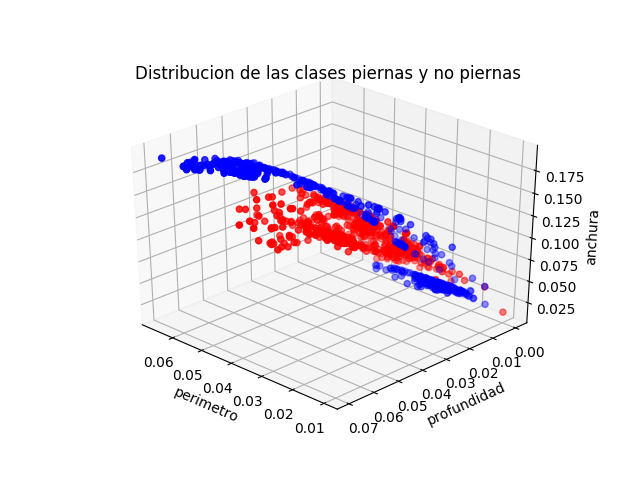
\includegraphics[scale=0.7]{img/plot3d-muchos-puntos}
\caption{Distribución de las clases. En azul ejemplos de la clase ``no pierna'', en rojo de la clase ``pierna''.}
\label{fig:3d}
\end{figure}

Podemos ver que, en general, las regiones que separan a los puntos están bastante
delimitadas. Vemos que también hay algunos puntos que son de la clase ``pierna''
que están mezclados con los de la otra clase. Por tanto, estos puntos se podrían
considerar como \textit{outliers}, y es muy posible que el clasificador no sea
capaz de clasificarlos correctamente, ya que son ruido.

Una vez que hemos comentado esto, vamos a ver qué resultados hemos obtenido al ejecutar
el programa. También comentaremos qué decisiones hemos tomado y el porqué de ellas:

\begin{scriptsize}
\verbatiminput{svm-25.log}
\end{scriptsize}

Lo primero que vemos son los resultados de validación. Ahí vemos que el
peor modelo es el que utiliza el \textit{kernel} lineal. Tiene una \textit{accuracy}
a muy próxima al 0.5, por tanto se podría casi considerar que clasifica de forma aleatoria.
Los \textit{kernels} polinómicos sí que son algo mejores. Parece que entre el grado 3 y
el 4 no hay mucha diferencia, ya que los resultados obtenidos son muy parecidos. El de
grado 2 se queda bastante por detrás, siendo por tanto el peor de los polinómicos.
Para sorpresa, el \textit{kernel} de base radial es el que obtiene los mejores
resultados, ya que obtiene una \textit{accuracy} de casi 0.9. Por tanto, en esta
primera comparación vemos que el \textit{kernel} radial es el mejor de entre los
probados.

Si ahora observamos los resultados para el conjunto de validación, vemos que en general son
parecidos a los obtenidos por validación, un poco por encima o por debajo de ellos, en general.
Vemos que de nuevo el \textit{kernel} lineal es el peor de todos ellos.
Observando su matriz de confusión vemos que clasifica bien todos los ejemplos positivos pero mal todos
los negativos. Por tanto, se puede directamente descartar este modelo, ya que lo hace
bastante mal en general. Si observamos los polinómicos, vemos que el mejor es el de grado
4, ya que es el que clasifica mejor, tiene una mayor \textit{accuracy} y unos mejores
valores de precisión y \textit{recall} en general. No obstante, parece que todos los
polinómicos tienen problemas serios con los casos negativos (cuando no es pierna), ya que se
equivocan demasiado (tienen un \textit{recall} muy bajo para los negativos).
Finalmente, si observamos los resultados ofrecidos por el \textit{kernel} de base radial,
vemos que los resultados son los mejores obtenidos hasta ahora en todas las métricas.
Es el que mejor clasifica tanto los ejemplos positivos como los negativos.
Por tanto, tal y como pasaba en el caso anterior, podemos afirmar que el \textit{kernel}
de base radial es el mejor modelo, y es el claro candidato a ser mejorado.

Una vez que se ha determinado el mejor modelo, se ha realizado una \texttt{GridSearchCV}
para obtener los mejores hiperparámetros. Se ha encontrado que el mejor valor de $C$ es 10.
Por tanto, una vez que se ha determinado este valor, como el clasificador ya estaba entrenado
para la mejor combinación de hiperparámetros, podemos estudiar su comportamiento con el
conjunto de validación.

Vemos que ha habido bastante mejora respecto al modelo base, ya que clasifica casi todos
los ejemplos positivos como piernas a excepción de uno, y falla solo unos pocos negativos. Vemos
además que todos los otros valores han mejorado, desde el \textit{accuracy} hasta la precisión
y el \textit{recall}. Por tanto, podemos afirmar que sí que ha merecido la pena
buscar los mejores hiperparámetros, ya que nos han perimitido mejorar bastante los resultados
obtenidos.

Con todo esto hecho, ahora podemos entrenar el modelo con todos los datos de los
que disponemos. De esta forma, los resultados obtenidos en el futuro muy posiblemente
serán mejores que los que podríamos obtener actualmente, ya que al tener más datos con los
que entrenar, el clasificador será capaz de generalizar mejor, ya que ha visto más situaciones
diferentes. Una vez hecho el último ajuste, guardamos los datos en un fichero utilizando
el módulo \texttt{joblib} de \texttt{sklearn}.

\section{Predicción y corrección de los datos}

Ahora que hemos entrenado el modelo, es hora de ponerlo a prueba con la escena
de test. Para ello, se ha creado el \textit{script} \textbf{predecir.py}, el cuál
se conecta al servidor de V-REP, lee los datos del laser, procesa la información y
obtiene los puntos, extraer los clusters, obtiene las características y predice
las clases de los objetos. Aparte, con lo que ha predicho, se muestra un gráfico, donde
se pueden ver los clusters obtenidos, a qué clase pertenecen y el punto medio de la línea
que une los centroides de dos clusters cercanos de la misma clase, representando la posición del objeto
detectado. Finalmente se cierra la conexion y se detiene la simulacion.

Para hacer todo esto, se han reutilizado muchas de las funciones anteriores, como la 
de iniciar y parar la conexion, la de procesar la lectura laser, la de obtener los
clústers y la de obtener las características. Adicionalmente, se han impelementado las
siguientes funciones:

\begin{itemize}[label=\textbullet]
	\item \texttt{calcular\_centroide}: Función que calcula el centroide de un cluster.
	\item \texttt{calcular\_centroides\_clusters}: Función que calcula el centroide de
	un grupo de clusters, juntándolos todos luego en un único \textit{array}.
	\item \texttt{calcular\_punto\_medio\_centroides}: Función que calcula el punto medio
	de los centroides de dos clusters próximos. Para hacerlo, se utiliza un \texttt{KDTree},
	es decir, un árbol multidimensional. Esta estructura de datos permite obtener
	los $k$ puntos más próximos a uno. Como vamos a buscar los puntos más próximos a los mismos
	que forman el árbol, tendremos que buscar para $k=2$ puntos, ya que el primer punto más cercano
	será él mismo. Una vez que tenemos los índices de los vecinos más cercanos, procesamos cada
	centroide. Se comprueba si el centroide más próximo es de la misma clase y, en caso de serlo,
	se calcula el punto medio entre los dos centroides y se añade a la lista. Además, al compartir la misma clase,
	se guarda la etiqueta del punto medio. Si se da el caso de que no son de la misma clase, se guarda
	el centroide actual en una lista aparte, además de su etiqueta. Esto será más útil más adelante,
	ya que esta información no se pintará de momento.
	\item \texttt{plot\_prediccion}: Funcion que pinta el gráfico mencionado anteriormente.
	\item \texttt{predecir}: Funcion que hace todo el proceso anteriormente descrito (detectar,
	obtener puntos, clusters, características, predecir y cálculo de los puntos medios).
\end{itemize}

Una vez explicada la funcionalidad básica, vamos a poner en funcionamiento el
programa. Vamos a coger la escena de test disponible y vamos a predecir las
clases de los objetos disponibles. A continuación podemos ver dicha escena:

\begin{figure}[H]
\centering
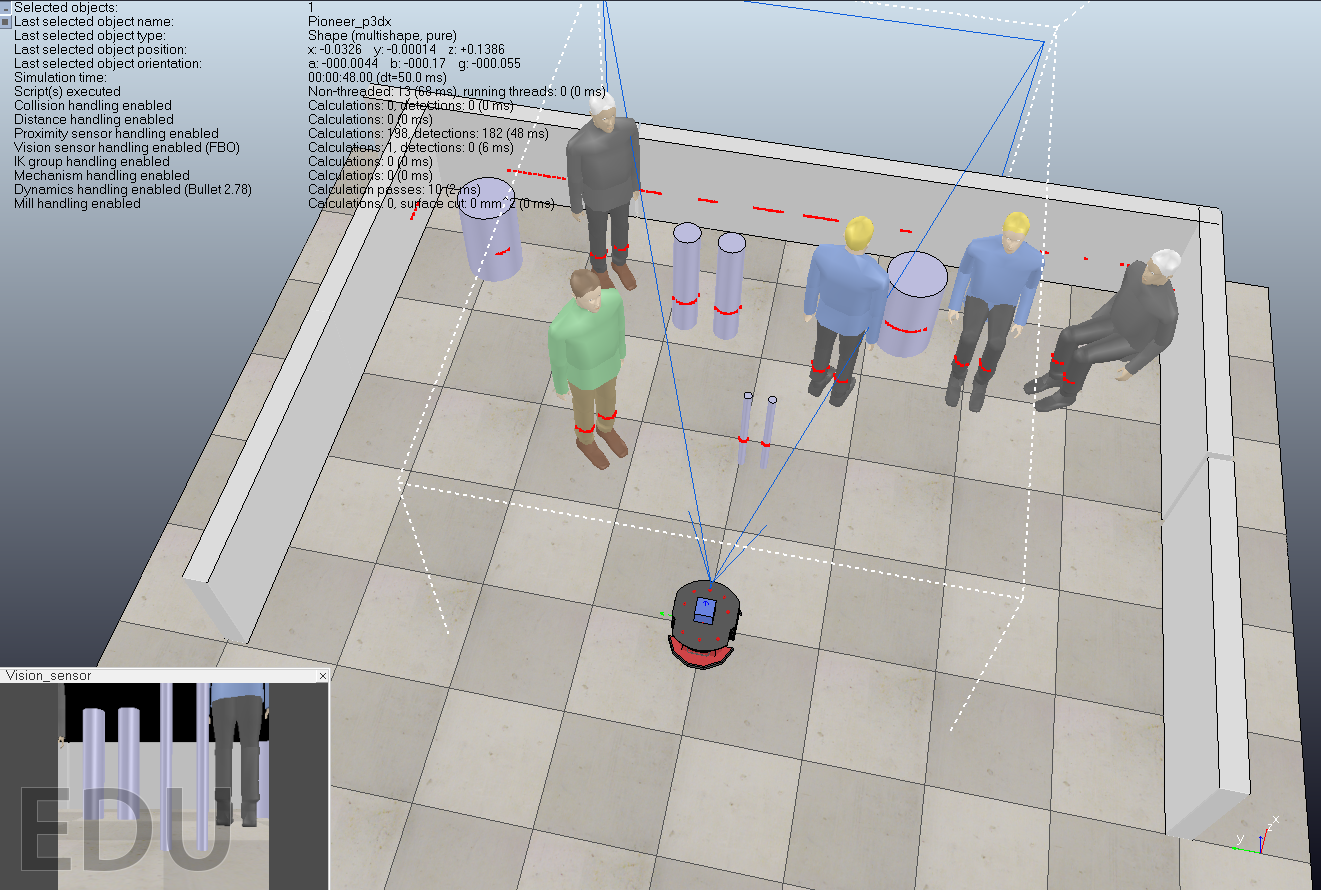
\includegraphics[scale=0.3]{img/simulador1}
\caption{Escena inicial de test.}
\end{figure}

Ejecutamos el programa y obtenemos los siguientes resultados:

\begin{figure}[H]
\centering
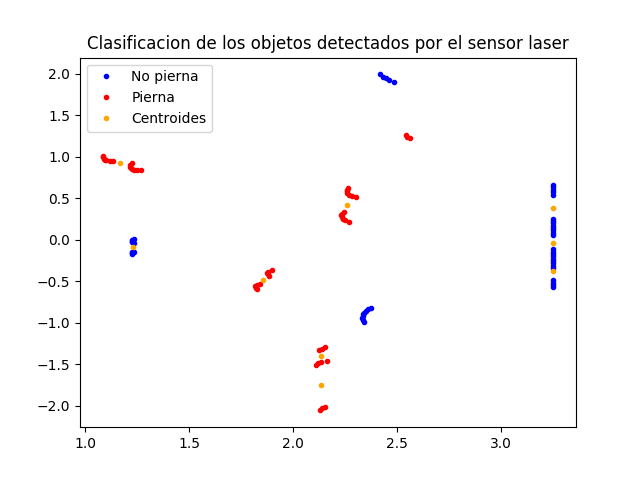
\includegraphics[scale=0.6]{img/pred1-mal}
\caption{Resultados de la predicción de la escena.}
\label{fig:pred1-mal}
\end{figure}

Como podemos ver en la figura \ref{fig:pred1-mal}, predice bien casi todos los
objetos menos el par de cilindros que están al fondo, entre la persona con el
jersey gris y la persona persona con el jersey azul. Podemos ver que esos dos
los clasifica como ``pierna'' en vez de como ``no pierna''. Además, parece que no
detecta la pared de la izquierda, y para la persona de la derecha del
todo solo detecta una pierna, haciendo que el punto medio del objeto esté entre
las dos personas sentadas. Sorprendentemente clasifica bien la pared, teniendo
en cuenta que hasta ahora nunca ha visto algo así.

A la vista de los resultados, podemos afirmar que estos no son del todo buenos,
ya que se esperaba que lo hiciese perfecto en la escena de test. Para intentar
mejorar los resultados, podemos hacer toda una serie de cosas, como tomar
más muestras, cambiar la forma en la que se generan los clusters, o intentar
mejorar más el clasificador, buscando por ejemplo una mejor combinación de hiperparámetros
que la que se tiene actualmente.

La solución que yo he propuesto consta de dos partes. Por una parte, se modifica
la forma de generar clusters. Ahora el número \textbf{máximo de puntos por cluster} es
de 13, y el \textbf{umbral de la distancia entre dos puntos consecutivos} es 0.05.
El número mínimo de puntos se queda igual. Estos valores se han obtenido tras realizar
bastantes pruebas, buscando cuál podría ser la mejor combinación de parámetros para la generación
de clusters. Por otra parte, he aumentado
el número de valores de $C$ que probar a la hora de buscar los mejores hiperparámetros.
He añadido valores más grandes, como 50 y 100, con el objetivo de penalizar más los
puntos que caen dentro del margen. Por tanto, he tenido que volver a agrupar los
puntos en clusters, generar de nuevo características y entrenar de nuevo. A la
hora de entrenar, si se visualizan los datos, se obtiene el siguiente gráfico:

\begin{figure}[H]
\centering
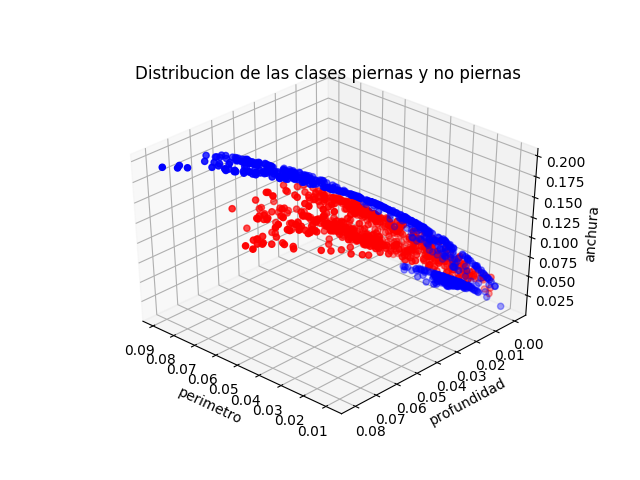
\includegraphics[scale=0.57]{img/plot3d-pocos-puntos}
\caption{Distribución de las clases. En azul ``no piernas'', en rojo ``piernas''.}
\end{figure}

Vemos que los puntos siguen más o menos la misma organización que la que se puede
ver en la figura \ref{fig:3d}, solo que esta vez parece que hay algo menos
de puntos que se puede dar que no se clasifiquen correctamente.

Si analizamos los resultados del entrenamiento, vemos lo siguiente:

\begin{scriptsize}
\verbatiminput{svm-13.log}
\end{scriptsize}

Los resultados son en general muy parecidos a los obtenidos antes, solo que ahora
el modelo con \textit{kernel} de base radial base (sin mejora de hiperparámetros)
es algo peor que en el caso anterior. A la hora de ajustar los hiperparámetros, vemos
que el mejor valor de $C$ es 100, y que la \textit{accuracy} obtenida es igual 
que en el caso anterior. La matriz de confusión indica que ahora se equivoca en menos
casos cuando no se trata de una pierna y un poco más cuando sí lo es, pero hay que considerar
que hay un mayor número de datos en el conjunto de validación. Observando los valores de precisión
y \textit{recall} vemos que son muy parecidos
a los obtenidos anteriormente, solo que están cambiados (para la clase para la que antes
la precisión era mejor, ahoa es peor, y lo mismo pasa con el \textit{recall}). Sin embargo,
su media sigue siendo la misma, y tampoco es que los valores obtenidos disten mucho de los
anteriores. Por tanto, en un principio, el modelo ofrecerá unos resultados igual de buenos
que el anterior.

Si ahora lo llevamos a la escena de test y repetimos el proceso, se obtiene la siguiente
predicción:

\begin{figure}[H]
\centering
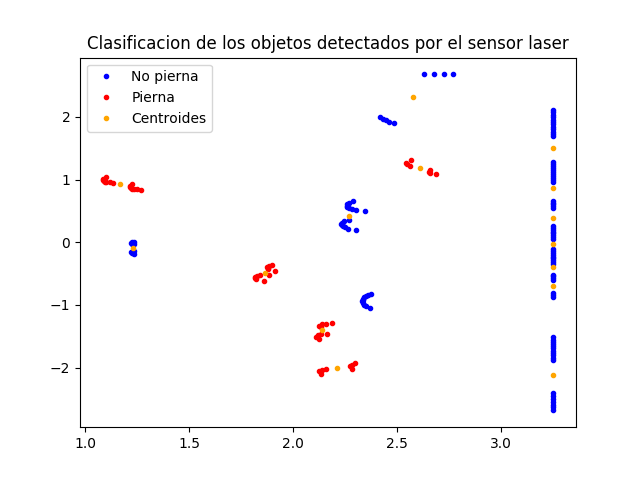
\includegraphics[scale=0.5]{img/pred1-bien}
\caption{Resultados de la predicción de la escena.}
\label{fig:pred1-bien}
\end{figure}

Vemos que ahora sí que clasifica los cilindros bien como ``no pierna''. Además, ahora
detecta también la pared izquierda, además de más puntos en la pared del fondo (las cuáles
sigue clasificando bien). Adicionalmente, detecta la pierna de la otra persona sentada a
la derecha del todo, estimando mejor por tanto el centro del objeto.

Por tanto, vemos que estos cambios, en un principio, han mejorado el modelo que teníamos
anteriormente.

Para comprobar si es bueno, vamos a cambiar la orientación del robot y vamos a predecir,
para ver qué tal se comporta. A continuación se pueden ver los resultados, junto con
la modificación a la escena realizada:

\begin{figure}[H]
\centering
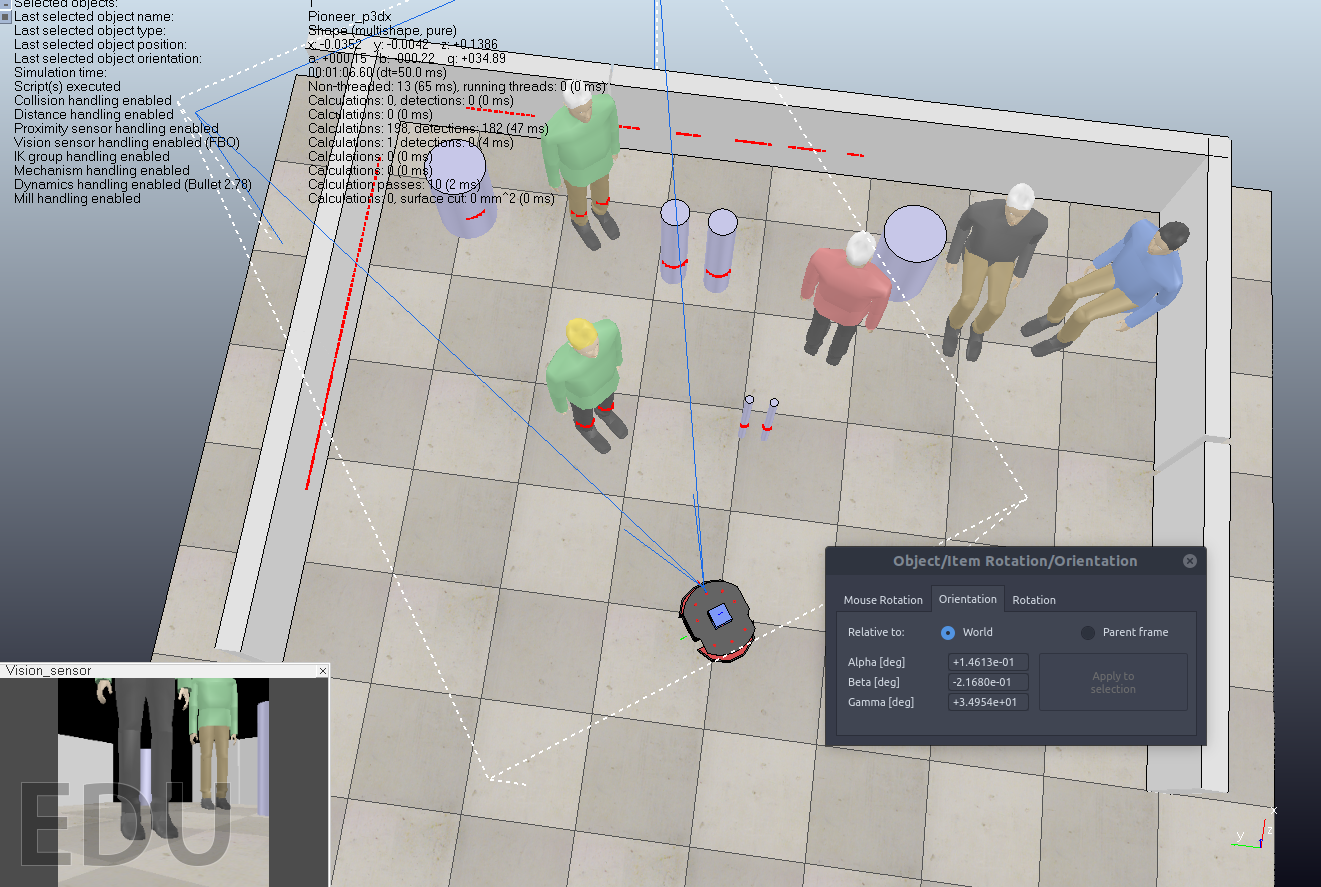
\includegraphics[scale=0.3]{img/simulador2}
\caption{Escena de test con rotación del robot a la izquierda.}
\end{figure}

\begin{figure}[H]
\centering
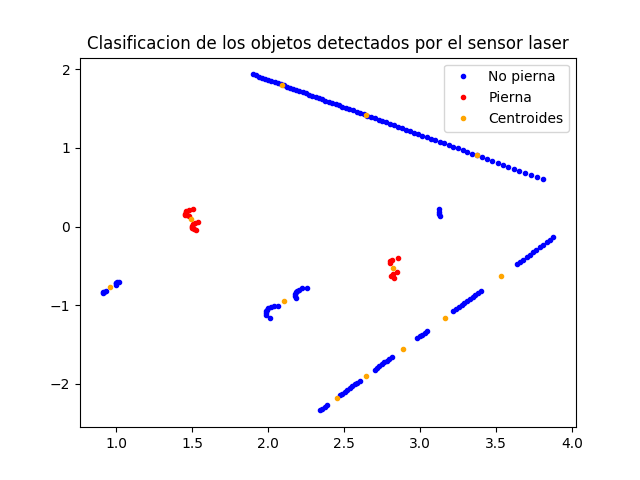
\includegraphics[scale=0.6]{img/pred2}
\caption{Resultados de la predicción de la escena anterior.}
\label{fig:pred2}
\end{figure}

\begin{figure}[H]
\centering
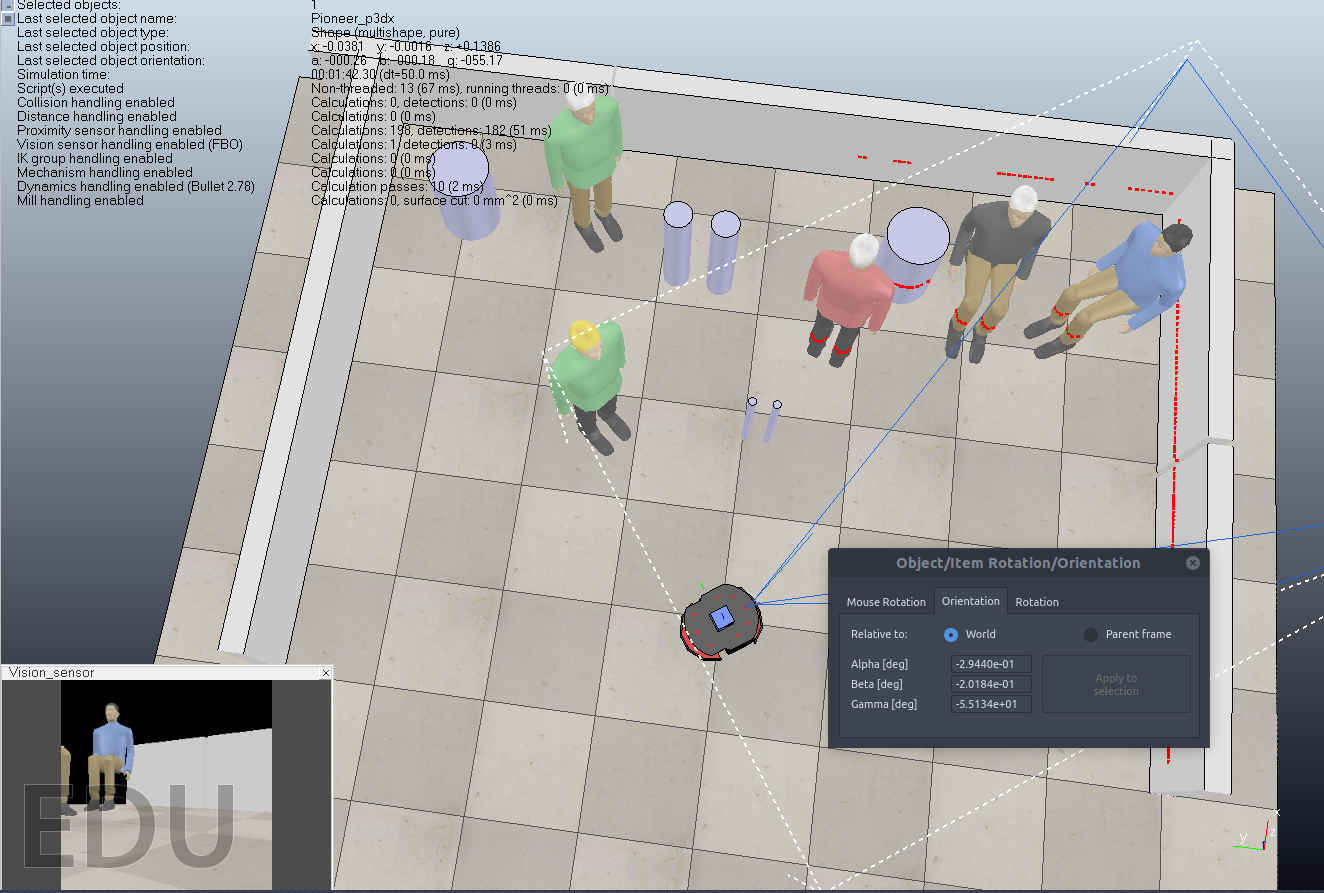
\includegraphics[scale=0.3]{img/simulador3}
\caption{Escena de test con rotación del robot a la derecha.}
\end{figure}

\begin{figure}[H]
\centering
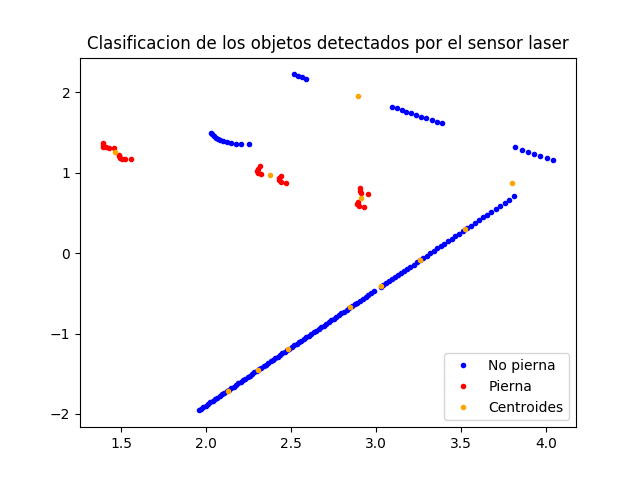
\includegraphics[scale=0.6]{img/pred3}
\caption{Resultados de la predicción de la escena anterior.}
\label{fig:pred3}
\end{figure}

Vemos que en los dos casos el modelo ha predicho todos los objetos correctamente. Por tanto
podemos afirmar con cierta certeza que nuestro modelo es bastante bueno, ya que es capaz de
clasificar correctamente los elementos de la escena de test, independientemente de la orientación
del robot. Para tener una certeza del 100\% de que lo hace bien, habría que probar todos
los posibles casos y, en caso de ver en algún momento algo no se detectase correctamente,
se podría probar a modificar la forma de generar los clusters o tomar más muestras.

\section{Apartado opcional: detección de objetos}

Una vez hecho todo lo anterior, se ha realizado la detección de los objetos de
la escena. El objetivo es detectar todos los objetos y crear una tabla en formato
\texttt{HTML} que visualice la clase real del objeto, la clase predicha por
el clasificador, la distancia al objeto y una imagen del objeto detectado.
Los objetos son tanto los puntos medios de la linea que une dos clusters próximos
como los centroides de los objetos no emparejados (recordemos la función para calcular
los puntos medios de la sección anterior, que también devolvía esa información).

Para hacer esta tarea, se ha creado el archivo \textbf{detectar.py}. Este archivo, igual
que el anterior, reutiliza ciertas funciones anteriores. En concreto, utiliza la función de
\texttt{predecir} y la de \texttt{capturar\_guardar\_imagen}, entre otras, como la de
iniciar la conexion y detener la simulacion y la conexion.

El funcionamiento principal del \textit{script} es conectarse con el servidor, obtener
\textit{handlers} para el robot y los motores derecho e izquierdo (aparte del de la
cámara que se tenía anteriormente), predecir, juntar los puntos medios obtenidos con los
centroides no emparejados y hacer lo mismo para las etiquetas (recordemos que tenemos que
detectar todos los objetos, incluso aquellos cuyos centroides no han podido ser emparejados con
otros), obtener las orientaciones
y los valores reales de los objetos (estos valores están insertados a mano en el \textit{script},
con lo cuál cualquier modificación a la escena va a hacer que los valores reales dejen de
ser válidos), ordenar las orientaciones y el resto de información en función de los
valores de las orientaciones, crear el directorio de salida de las imagenes, rotar
el robot a cada orientacion y capturar la imagen de la cámara y generar el fichero \texttt{HTML}
de salida. Finalmente, se cierra la conexión y la simulación.

De lo explicado anteriormente, hay algunos puntos a destacar:

\begin{enumerate}
	\item Para hacer las rotaciones se ha utilizado la función \texttt{simxSetObjectOrientation}.
	Esta función modifica directamente la orientación de los objetos referenciados por los \textit{handlers}
	a la orientación especificada. Para especificar la orientación, se tiene que utilizar el formato
	de coordenadas de Euler, las cuáles son $\alpha$ (rotación en el eje $X$), $\beta$
	(rotación en el eje $Y$) y $\gamma$ (rotación en el eje $Z$). Como nos interesa rotar
	el robot en el eje $Z$, solo especificaremos valores para $\gamma$, dejando el resto a 0.
	\item Todas las rotaciones están especificadas en radianes, ya que es el formato que acepta
	V-REP.
	\item El motivo de obtener los \textit{handlers} de los motores es que también
	se rotarán estos, ya que si solo se rota el robot, la cámara se inclina un poco hacia
	un lado, haciendo que las capturas que se tomen posteriormente estén algo inclinadas.
	\item El motivo por el que se ordenan las orientaciones y el resto de datos no tiene
	mucha importancia. Simplemente se hace para que todas las capturas de la cámara se puedan
	tomar en una sola pasada, sin tener que volver hacia atrás en ningún momento.
\end{enumerate}

Una vez dicho esto, vamos a comentar brevemente las funciones implementadas en este
archivo, las cuáles son utilizadas para completar la tarea de generación de resultados:

\begin{itemize}[label=\textbullet]
	\item \texttt{rotar\_robot}: Función que rota el robot y los motores hasta situarlos
	en $\gamma$ grados. Al final, espera un segundo para evitar fallos de comunicación
	con el servidor (si se hace demasiado rápido la actualización no da tiempo a que se haga
	correctamente).
	\item \texttt{calcular\_distancias\_objetos}: Función que calcula la distnacia del robot
	a un conjunto de objetos.
	\item \texttt{calcular\_orientaciones}: Función que calcula las orientaciones. Para calcular
	las orientaciones, primero calcula las distancias a los objetos. A continuación, se llevan
	dichos puntos al eje $X$ (haciendo que su coordenada $y$ valga 0) y se calcula la distancia
	hasta cada uno de ellos. De esta forma, se tienen dos lados de un triángulo rectángulo para
	cada objeto detectado, de forma que la hipotenusa está formada por la línea que va del robot
	al objeto en cuestión, y uno de los catetos es el que va del robot al punto trasladado sobre
	el eje $X$ del objeto en cuestión. Utilizando las dos distancias anteriores se puede calcular
	el coseno, y para sacar el valor de $\gamma$, la orientación, solo hace falta aplicar la
	función arco coseno. Todas las orientaciones calculadas son positivas; es decir, están en el
	primer cuadrante. No obstante, en algunos casos tienen que ser negativas, ya que hay objetos
	en el cuarto cuadrante. Por tanto, hay que cambiar los valores de dichas orientaciones
	a negativo en los casos en los que el objeto detectado quede a la derecha del robot, es decir,
	donde la coordenada $y$ del objeto sea negativa.
	\item \texttt{escribir\_comienzo\_fichero}: Función que escribe el comienzo del fichero.
	\item \texttt{escribir\_fila}: Función para escribir una fila de la tabla con el formato
	antes especificado.
	\item \texttt{escribir\_final\_fichero}: Función para escribir el final del archivo.
\end{itemize}

Los resultados se pueden ver en el archivo \textbf{resultados.html}, donde se puede
ver la tabla con el formato anteriormente mencionado para cada uno de los objetos
detectados de la escena.

\end{document}

